

	\begin{frame}{Master-Worker}
		\centerline{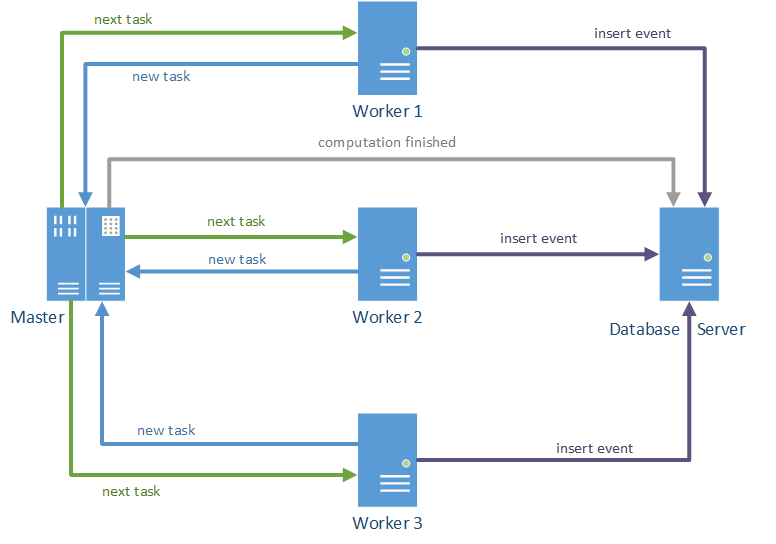
\includegraphics[scale=0.5]{images/master}}
	\end{frame}
	\begin{frame}{Task Stealing}
		\centerline{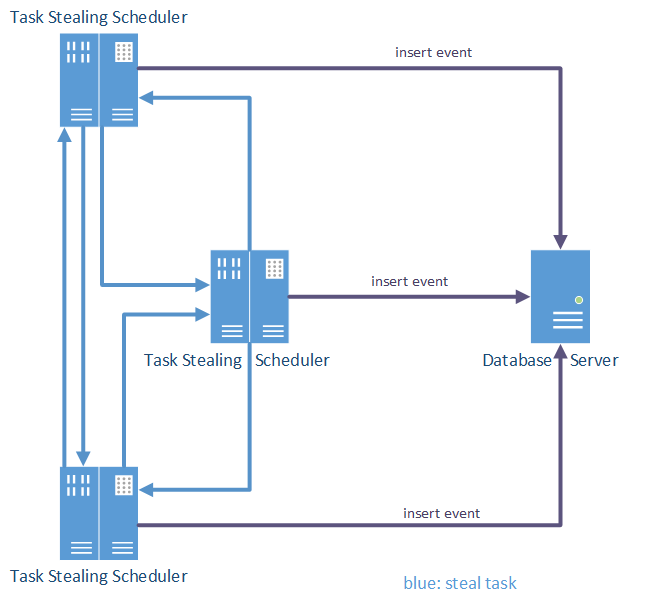
\includegraphics[scale=0.5]{images/taskstealing}}
	\end{frame}

	\begin{frame}{Scheduling Strategies}
	\begin{minipage}[]{.7\textwidth}%
			\begin{itemize}
		\item<2-> Non-statistical
		\begin{itemize}
			\item<3-> First In-First Out (FIFO)
			\item<4-> Last In-Fist Out (LIFO)
		\end{itemize}
		\item<5-> Statistical
		\begin{itemize}
			\item<6-> Shortest Job First (SJF)
			\item<7-> Longest Job First (LJF)
		\end{itemize}
		\item<8-> Standardized interface 
			\begin{itemize}
				\item<9-> simple to include new strategies
			\end{itemize}					
		\end{itemize}
\end{minipage}%
\begin{minipage}[]{.3\textwidth}%
  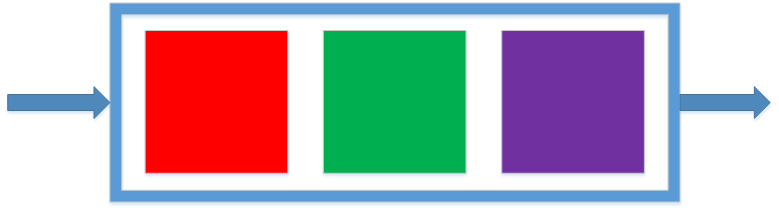
\includegraphics[width=\textwidth]{images/fifo}%
\end{minipage}		
		
	\end{frame}
	\begin{frame}{Master-Worker vs. Task Stealing}
		\begin{itemize}
			\item<2-> Master-Worker
				\begin{itemize}
					\item<3-> fast standard c++ implementation
					\item<4-> dynamic size
					\item<5-> easy to switch between scheduling strategies at runtime	
				\end{itemize}
			
			\item<6-> Task stealing
					\begin{itemize}
						\item<7-> custom implementation inside a MPI-Window
					\end{itemize}
			
		\end{itemize}
	\end{frame}